\subsection{沉砂池}
\subsubsection{沉砂池的选择}
在这次处理含有高浓度有机物质的污水的沉砂池设计中(详见表 \ref{tab:in water}),传统的平流沉砂池和竖流沉砂池效果不佳,无法有效去除这些有机物质,增加了后续处理的困难。相比之下,曝气沉砂池结合曝气和沉砂的特点,具有多个优势。它引入气体曝气系统,提供溶解氧,促进微生物生长和活性,加快有机物的降解速率。即使有机物含量高,曝气沉砂池也能更有效地降解它们。此外,曝气沉砂池能够更好地实现悬浮物固液分离,通过增加悬浮物的浮力,使其更容易上升到水面形成浮泡,从而减少悬浮物含量,改善处理效果。此外,曝气沉砂池对处理面积需求小且能耗低。相比传统的平流沉砂池和竖流沉砂池,在相同处理效果下,曝气沉砂池占地面积更小,适用于城镇污水处理厂设计。同时,曝气设备的能耗较低,降低了运行成本。综上,我们选择了曝气沉砂池。\cite[pp.75-87]{《污水处理厂工艺设计手册》}


\subsubsection{曝气沉砂池的计算}
查阅张辰主编的《污水厂设计》,曝气沉砂池设计计算公式如下表 \ref{tab:Aeration grit tank design calculation formula} 所示:
\begin{table}[H]
	\centering
	\caption{曝气沉砂池设计计算公式\cite[p.161]{《污水厂设计》}}
	\begin{tabular}{l|l|l}
		\toprule
		名称    & 公式    & 符号说明 \\
		\midrule
		水池总有效容积 & $V=Q_{max}t\times60$ & \makecell[l]{$V$——水池总有效容积,m$^3$;\\ $Q_{max}$——最大设计流量,m$^3$/s;\\ $t$——最大设计流量时的流行时间,min} \\
		\midrule
		水流断面积 & $A =\dfrac{Q_{max}}{v_1}$ & \makecell[l]{$A$——水流断面积,m$^2$;\\$v_1$——最大设计流量时的水平流速,m/s,\\\phantom{$v_1$——}一般采用 $0.06\sim0.12$ m/s} \\
		\midrule
		池总宽度  & $B=\dfrac{A}{h_2}$   & \makecell[l]{$B$——池总宽度,m;\\$h_2$——设计有效水深,m} \\
		\midrule
		池长    & $L=\dfrac{V}{A}$   & $L$——池长,m \\
		\midrule
		每小时所需空气量 & $q=dQ_{max}\times3600$ &  \makecell[l]{$q$——每小时所需空气量,m$^3$/h;\\$d$——每立方米污水所需空气量(m$^3$/m$^3$)} \\
		\bottomrule
	\end{tabular}%
	\label{tab:Aeration grit tank design calculation formula}%
\end{table}%

\begin{figure}[H]
	\centering
	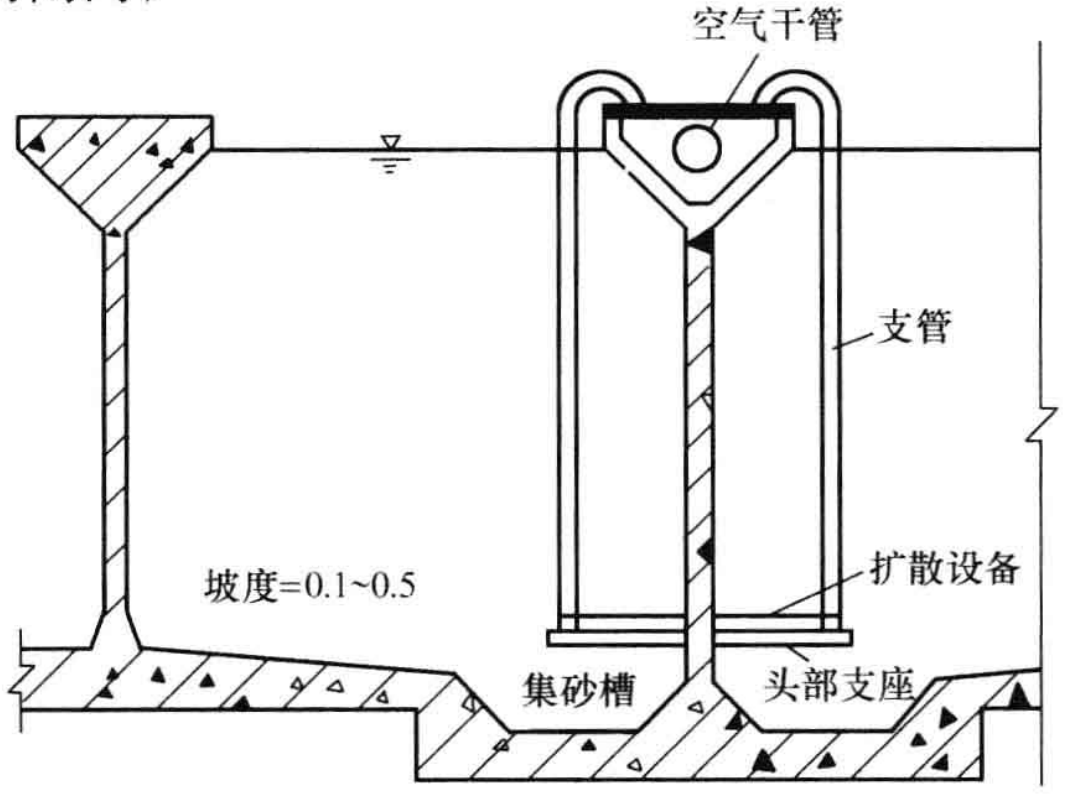
\includegraphics[width=0.6\textwidth]{figures/Sketch of the appearance of the aeration grit tank.png}
	\caption{曝气沉砂池外型草图}
	\label{fig:Sketch of the appearance of the aeration grit tank}
\end{figure}

\begin{enumerate}
	\item 池子总有效容积
	
	设 $t=2$ min\footnote{最大流量时停留时间为 $1\sim3$ min。\cite[p.30]{《城市污水厂处理设施设计计算(第三版)》}},因为曝气沉淀池的个数为2,所以单个曝气沉淀池的总有效容积为:
	\begin{align}
		V=Q_{max}t\times60 =\dfrac{0.672}{2}\times2\times60\;\text{m$^3$} =\eval{\dfrac{0.672}{2}\times2\times60}[3]\;\text{m$^3$}
	\end{align}
	
	\item 水流断面面积

	设$v_1=0.06$ m/s\footnote{由表 \ref{tab:Aeration grit tank design calculation formula} 可知,最大设计流量时的水平流速$v_1$,一般采用 $0.06\sim0.12$ m/s;《室外排水设计标准》(GB 50014-2021)中提到水平流速不宜大于0.l m/s。},所以单个曝气沉淀池的水流断面面积为:
	\begin{align}
		A =\dfrac{Q_{max}}{v_1} =\dfrac{0.672}{2}\times\dfrac{1}{0.06} \;\text{m$^2$} =\eval{\dfrac{0.672}{2}\times\dfrac{1}{0.06}}[3]\;\text{m$^2$}
	\end{align}

	\item 池总宽度

	设$h_2=2.0$ m\footnote{有效水深宜为 $2.0\sim3.0$ m。\cite[p.48]{GB500142021}},所以单个曝气沉淀池的池总宽度为:
	\begin{equation}
		B=\dfrac{A}{h_2}=\dfrac{5.6}{2.0} \;\text{m} =\eval{\dfrac{5.6}{2.0}} \;\text{m}
	\end{equation}

	池子格数设计为 $n=1$ 格,则每个池子宽度为:
	\begin{equation}
		b=\dfrac{B}{n}=\dfrac{2.8}{1}\;\text{m}=2.8 \;\text{m}
	\end{equation}
	所以宽深比:$\dfrac{b}{h_2}=\dfrac{2.8}{2.0}=1.4$,满足《室外排水设计标准》(GB 50014-2021)中曝气沉砂池的设计宽深比宜为$1.0\sim1.5$的要求。

	\item 池长

	单个曝气沉淀池的池长为
	\begin{equation}
		L=\dfrac{V}{A}=\dfrac{40.32}{5.6} \;\text{m} = \eval{\dfrac{40.32}{5.6}}[3] \;\text{m}
	\end{equation}

	\item 每小时所需氧气量

	设$d=0.1$ m$^3$\footnote{处理每立方米污水的曝气量为$0.1\sim 0.2$ m$^3$空气。\cite[p.30]{《城市污水厂处理设施设计计算(第三版)》}},所以单个曝气沉淀池的每小时所需氧气量为:
	\begin{align}
		q=dQ_{max}\times3600&=0.1\times\dfrac{0.672}{2}\times3600\;\text{m$^3$/h} \\
		&=\eval{0.1\times\dfrac{0.672}{2}\times3600}\;\text{m$^3$/h} \notag
	\end{align}

	\item 沉砂室沉砂斗体积(理论)
	\begin{equation}
		V=\dfrac{Q_{max}XT\times86400}{K_z \cdot 10^6}
	\end{equation}
	$X$——城镇污水沉砂量,m$^3$/10$^6$m$^3$污水;\par
	$T$——清除沉砂的间隔时间,d;\par
	$K_z$——污水流量总变化系数,$K_z=1.66$。

	取 $X=30$ m$^3$/10$^6$m$^3$污水\footnote{《室外排水设计标准》(GB 50014-2021):污水的沉砂量可按 0.03 L/m$^3$ 计算。},$T=2$ d\footnote{《室外排水设计标准》(GB 50014-2021):砂斗容积不应大于 2d 的沉砂量。},带入计算得:
	\begin{align*}
		V=\dfrac{Q_{max}XT\times86400}{K_z \cdot 10^6} &=\dfrac{\dfrac{0.672}{2}\times 30\times 2\times 86400}{1.66 \times 10^6} \;\text{m$^3$} \\
		& = \eval{\dfrac{0.672/2\times 30\times 2\times 86400}{1.66 \times 10^6}}[3] \;\text{m$^3$}
	\end{align*}

	\item 沉砂室沉砂斗体积(实际)
	
	\begin{figure}[H]
		\centering
		\begin{tikzpicture}[scale=1.5]
			% 绘制主体
			\draw (-2,0.8) rectangle (2,3.8);
			\draw (-2,2.8) -- ++(4,0);
			% 标记主体
			\foreach \x in {-2,2} {
				\draw (\x,4) -- ++(0,0.2);
			}
			\draw[stealth-stealth] (-2,4.1) -- ++(4,0) node[midway, above] {$b$};
			\foreach \y in {0,0.8,2.8,3.8} {
				\draw (2.2,\y) -- ++(0.2,0);
			}
			\draw[stealth-stealth] (2.3,0) -- ++(0,0.8) node[midway, right] {$h_3$};
			\draw[stealth-stealth] (2.3,0.8) -- ++(0,2) node[midway, right] {$h_2$};
			\draw[stealth-stealth] (2.3,2.8) -- ++(0,1) node[midway, right] {$h_1$};
			% 绘制漏斗
			\foreach \x in {30} {
				\draw (0,0) -- ++(-0.15,0) -- ({180-\x}:0.6) -- (-2,0.8);
				\draw (0,0) -- ++(0.15,0) -- (\x:0.6) -- (2,0.8);
				% 绘制漏斗标记
				\draw ({180-\x}:0.6) ++(0,0.05) -- +(0,0.2);
				\draw (\x:0.6) ++(0,0.05) -- +(0,0.2);
				\draw[stealth-stealth] (0,0) ++(\x:0.6) ++(0,0.15) -- ++(-1.03,0) node[midway, above] {$a$};
				\draw ({180-\x}:0.6) ++(-0.5,0) -- ++(-0.2,0);
				\draw (0,0) -- ++(-1.22,0);
				\draw[stealth-stealth] ({180-\x}:0.6) ++(-0.5,0) ++(-0.1,0) -- (-1.12,0) node[midway, left] {$h_3'$};
				\draw ({180-\x}:0.4) arc ({180-\x}:180:0.4) node[midway, left] {$\alpha$};
			}
			% 标记漏斗
			\foreach \x in {-0.15,0.15} {
				\draw (\x,-0.2) -- ++(0,-0.2);
			}
			\draw[stealth-stealth] (-0.15,-0.3) -- ++(0.3,0) node[midway, below] {$a_1$};
			\foreach \x in {-0.15,0.15} {
				\draw (\x,-0.2) -- ++(0,-0.2);
			}
			\draw[stealth-stealth] (-0.15,-0.3) -- ++(0.3,0) node[midway, below] {$a_1$};
			\draw (2,0.8) ++(-0.8,0) arc (180:200:0.8) node[midway, left] {$\beta$};
		\end{tikzpicture}
		\caption{曝气式沉砂池计算草图}
		\label{fig:Sketch of an aeration grit tank}
	\end{figure}
	设沉砂斗为沿池长方向的梯形断面渠道(如上图 \ref{fig:Sketch of an aeration grit tank}),沉砂斗体积为
	\begin{equation}
		V_0=\dfrac{a+a_1}{2}\cdot h_3 L
	\end{equation}
	设沉砂池底部梯形的坡角为 $\alpha=55^{\circ}$\footnote{《室外排水设计标准》(GB 50014-2021):当采用重力排砂时,砂斗斗壁和水平面的倾角不应小于$55^{\circ}$。},沉砂室坡向沉砂斗的坡度 $\beta=15^{\circ}$\footnote{沉砂室坡向沉砂斗的坡度 $i=\tan{\beta}=0.1\sim 0.5$。\cite[p.31]{《城市污水厂处理设施设计计算(第三版)》}(此时 $\tan{\beta}=\tan{15^{\circ}}=\eval{\tan{15/180*\pi}}[4]$)},沉砂斗高度为 $h_3'=0.3$ m,沉砂斗窄口宽度为 $a_1=0.5$ m,则沉砂斗宽口宽度为
	\begin{align}
		a=\dfrac{2h_3'}{\tan{\alpha}}+a_1 = \dfrac{2\times 0.3}{\tan{55^{\circ}}}+0.5 \;\text{m} = \eval{\dfrac{2\times 0.3}{\tan{55/180*\pi}}+0.5}[3] \;\text{m}
	\end{align}
	又因为
	\begin{align}
		h_3=h_3'+\dfrac{B-a}{2}\tan{\beta} = 0.3+\dfrac{2.8-0.92}{2}\times \tan{15^{\circ}} \;\text{m} = \eval{0.3+\dfrac{2.8-0.92}{2}\times \tan{15/180*\pi}}[2] \;\text{m}
	\end{align}
	所以沉砂斗体积为
	\begin{align}
		V_0=\dfrac{a+a_1}{2}\cdot h_3 L = \dfrac{0.92+0.5}{2}\times 0.55 \times 7.2 \;\text{m$^3$} = \eval{\dfrac{0.92+0.5}{2}\times 0.55 \times 7.2}[3] \;\text{m$^3$}
	\end{align}
\end{enumerate}

% 查阅《室外排水设计标准》(GB 50014-2021),安全⽔头应大于 0.3 m,有效水深宜为$2.0$ m $\sim$ 3.0 m。则取 $h_1=0.5$ m,$h_2=2$ m。所以单个曝气沉砂池高度为
% \begin{equation}
% 	H=h_1+h_2+h_3=0.5+2+0.55 \;\text{m} = \eval{0.5+2+0.55} \;\text{m}
% \end{equation}


